\section{More Fun with Binary Stars}

\makelabheader

\bigskip

An astronomer observes the spectrum of a star many times over a series of days.
She observes that the H$\alpha$ line of hydrogen usually appears split
into two lines with slightly different wavelengths. She measures
the wavelengths of those two lines during each of her observations
and plots a graph of the results that looks like this:

\centerline{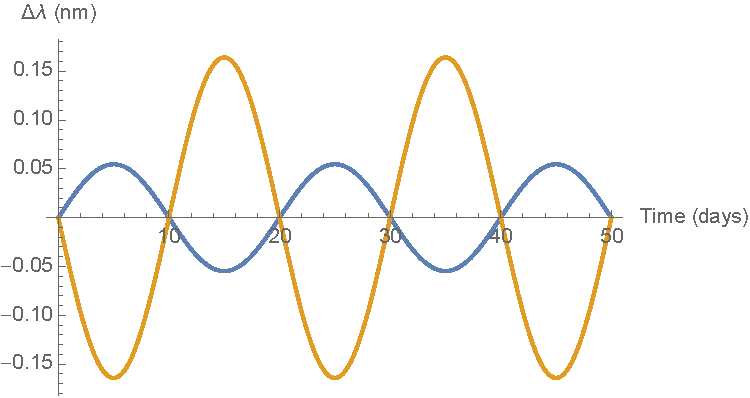
\includegraphics[width=5in]{binarycalcs/binary1.pdf}}

What's plotted on this graph are the wavelength shifts of the spectral line.
So when $t=0$ days, there is no shift at all, and both lines appear right
where they would be in the lab. A day or two later, the spectral line is split
in two, with one line (represented by the blue curve) having a wavelength slightly longer than expected, and one (represented by the yellow curve)
having a wavelength slightly shorter than expected. By 10 days, the two
spectral lines have come back together again, and then they split apart again.

As you probably know, the reason this is happening is that this star
is really a \textit{double-line spectroscopic binary system}. The two graphs
show the spectral lines due to the two stars in the system, which alternately
move toward you and away from you as they orbit around each other.

To save you the trouble of reading numbers off the graph, I'll
tell you that when $t=5$ days, the blue curve is at a height of 0.055 nm,
and the yellow curve is at $-0.16$ nm. This moment is when the two graphs
are at their highest and lowest points, meaning that one star is
moving directly toward you and one is moving directly away from you.
You can assume that the stars are moving in circular orbits.


Let's
call the star whose spectral line is given by the blue curve star number
1, and the other one star number 2. The wavelength of the H$\alpha$ line, 
when measured in the lab, is 656.3 nm. 
Armed with this information, I want you to tell me the following
about these stars and their orbits. 
(You may need some unit conversions. If so, look them up.)

\begin{enumerate}
\item How fast are the two stars moving?

\answerspace{2in}

\item Which star is heavier? What is the ratio of their masses $M_1/M_2$?
(Remember that the masses and speeds of the orbits are related,
so that $M_1v_1=M_2v_2$.)

\answerspace{1.5in}

\item What is the period of the orbit? (That is, how much time does
it take for the graph to repeat itself?)

\answerspace{1in}

\item What are the radii of the two stars' orbits? (Suggestion: 
How far does each star travel during one period of its motion? How
is that number related to the radius?)

\answerspace{1.5in}

\item At the end of this document is a picture of the two stars' orbits. 
You, the observer, are way off to the left. Say both stars
are moving counterclockwise.
When $t=5$ days, where are the two stars in this diagram? (Hint:
is star 1 moving toward you or away from you at this moment? What about
star 2?)
Mark the locations on the diagram with a ``5''.

\item Mark the locations of the two stars when $t=10,15$, and 20 days.
\item What is the distance between the two stars at any given time?
(Hint: How is it related to the radii of the two orbits, which you know?)
The distance between the two stars is the $a$ in Kepler's Third Law.

\answerspace{1in}

\item What is the total mass $M_1+M_2$?

\answerspace{1in}
\item What are the masses $M_1$ and $M_2$?
\end{enumerate}

\centerline{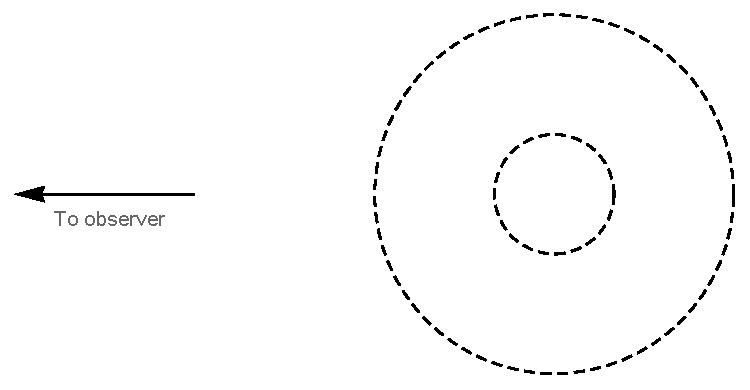
\includegraphics[width=4in]{binarycalcs/binary2.pdf}}

%% \vfil

%% {\bf Answers} (without all the detailed steps, and skipping the ones whose 
%% answers are pictures, because I'm lazy):

%% 1. $v_1=\SI{25000}{m/s}$, $v_2 = \SI{73000}{m/s}$.

%% 2. $M_1/M_2 = 2.9$.

%% 3. 20 days.

%% 4. $r_1=\SI{6.8e9}{m}$, $r_2 = \SI{2.0e10}{m}$.

%% 7. \SI{2.7e10}{m}.

%% 8. $1.95M_\odot$.

%% 9. $M_1 = 1.45M_\odot, M_1=0.5M_\odot$.


